\vspace{-1em}
\section{方法}
\label{sec:method}
\vspace{-0.5em}



\subsection{问题设定}
\vspace{-0.5em}
给定一张 RGB 图像 $\mathbf{I}$ 和用户提供的提示 $p$（掩码、框或点），我们的目标是在整个视频序列中识别同一对象并保持一致分割，避免跨帧错误对应或身份切换。
以往方法通常难以实现这一目标。
\textbf{基于 2D 的方法}（例如 SAM2~\cite{ravi2024sam2}）仅依赖外观特征，因此对视角或距离变化敏感，并容易在视觉相似对象之间混淆~\cite{videnovic2025distractor}，在较长序列中频繁跟踪失败。
\textbf{基于 3D 的方法}（例如 Mask3D~\cite{schult2022mask3d}、OpenYOLO3D~\cite{boudjoghra2024open}、EmbodiedSAM~\cite{xu2024esam}）通过 3D 掩码提议或结合相机位姿的稠密 2D 掩码来定位对象，但需要 SfM 或类似流程；随着帧数增加，其运行时间和复杂度快速增长，难以用于长序列。
另一种选择是在预测几何（例如 MUSt3R 的点云）上应用 3D 分割模型。然而，几何质量，尤其在动态场景中，会限制下游分割可靠性。此外，当前 3D 分割模型多为离线模型，不适合机器人导航等实时场景。更重要的是，2D 视频领域拥有更丰富的大规模训练数据，而我们采用的 SAM2 提供了强大的可提示 2D 先验，当前 3D 替代方案难以匹配。我们的方法利用这一优势，仅将 3D 信息作为轻量级关联线索，而非硬性前提，从而保持 2D 分割框架。具体而言，我们鼓励几何一致的特征匹配，使模型能够通过识别对象在 3D 空间中的对应关系来定位同一对象。


\vspace{-0.5em}
\subsection{架构}
\vspace{-0.5em}
整体流程如 \cref{fig:pipline} 所示。
对于每个视频帧 $i$，我们的模型提取两条互补特征流，分别捕获外观线索和多视角几何一致性。
首先，帧经过 SAM2 视觉编码器，产生 2D 外观特征图 $F_{\mathrm{2D}}^{i}$。
与此同时，同一帧输入 MUSt3R，后者通过其内部交叉注意力机制关注自身的多视角记忆，得到几何感知特征图 $F_{{3D}}^{i}$。随后，$F_{{2D}}^{i}$ 与 $F_{{3D}}^{i}$ 被融合为细化表示 $F_{{merged}}^{i}$。融合特征经过记忆注意力模块和掩码解码器处理，最后由记忆编码器编码为供未来帧引用的记忆特征。不同记忆选择方法的比较见 \cref{tab:memory-selection}。


\vspace{-1em}
\subsubsection{特征融合。}

\begin{figure*}[t]
  \centering
\vspace{-3mm}
  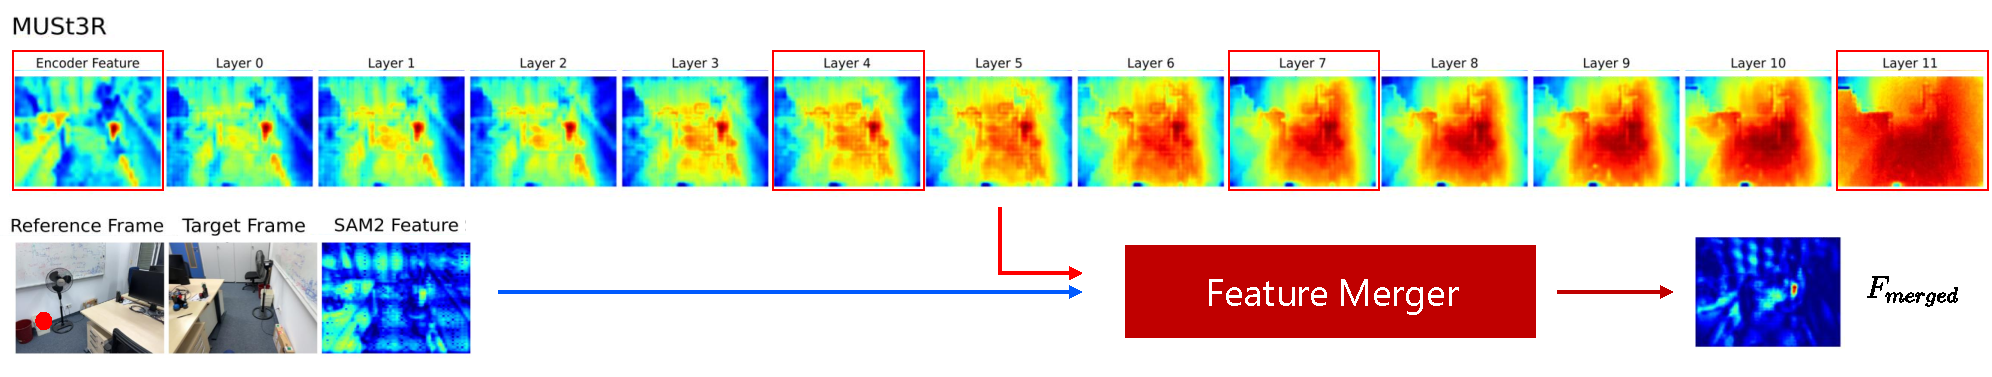
\includegraphics[width=\linewidth]{figs/FeatureMerging.pdf}
  \vspace{-6mm}
  \caption{\textbf{用于特征融合的特征示意。} 热力图由红色查询点与目标帧之间的余弦相似度计算得到。如底行所示，原始 SAM2 在大幅视角变化下失败。相反，随着 MUSt3R 特征层级从语义对应逐渐转向点云域，我们选择中间层以同时保留语义相关性和几何结构。通过将 MUSt3R 的几何线索与 SAM2 的视觉语义结合，融合特征 $F_{{merged}}$ 能更可靠地定位目标对象。
  }
  \label{fig:feature_merging}
\vspace{-3mm}
\end{figure*}

MUSt3R 特征在不同层级包含不同信息：浅层更偏局部纹理，中间层同时保留语义和几何对应，深层则更接近重建所需的点云表示。我们发现，中间层最适合对象跟踪，因为它们既具备跨视角几何稳定性，又不完全丢失对象级语义。于是，我们从多个 MUSt3R 层级提取特征，并通过轻量级 Feature Merger 将它们与 SAM2 的外观特征结合。

给定 SAM2 特征 $F_{\mathrm{2D}}^{i}$ 和 MUSt3R 特征 $F_{\mathrm{3D}}^{i}$，Feature Merger 首先使用交叉注意力将几何线索注入 2D 表示，然后通过卷积细化融合结果。得到的 $F_{\mathrm{merged}}^{i}$ 继承了 SAM2 的可提示分割能力，同时获得了 MUSt3R 编码的几何对应关系。由于 MUSt3R 只在推理时从 RGB 帧提取特征，整个系统无需相机位姿、深度图或显式 3D 重建后处理。

\vspace{-0.5em}
\subsection{训练帧采样}
\label{subsec:sampling}
\vspace{-0.5em}

\begin{figure*}[t]
  \centering
  \begin{minipage}{0.32\textwidth}
    \centering
    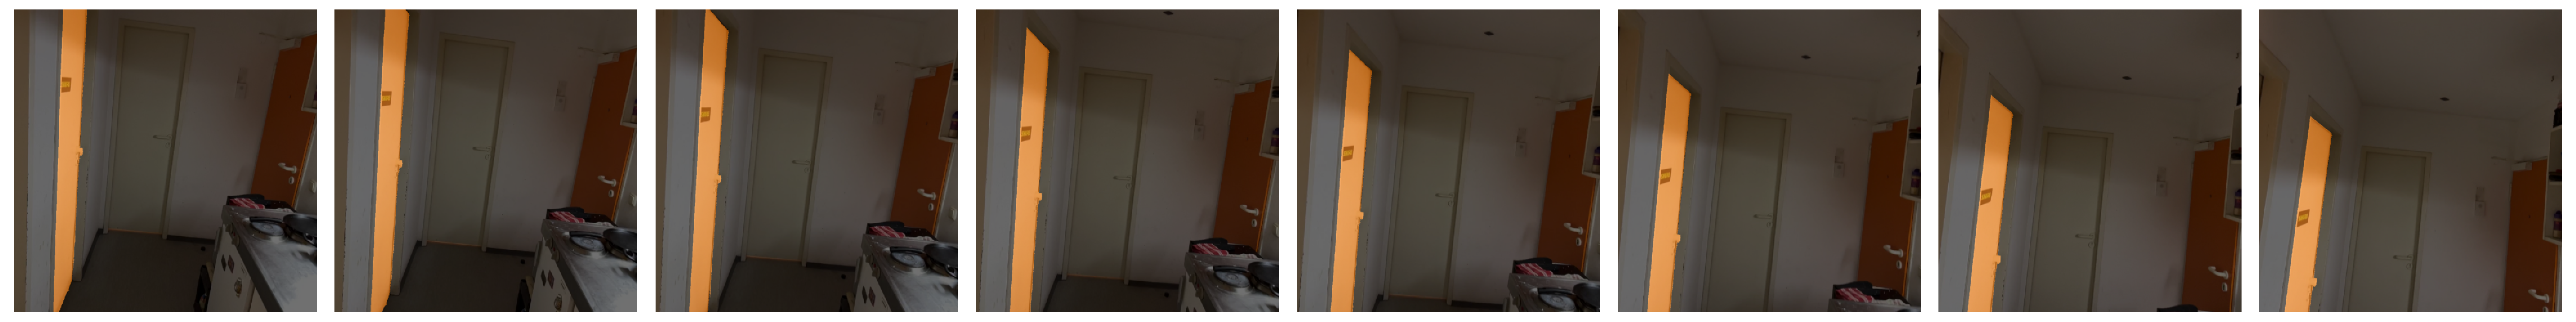
\includegraphics[width=\linewidth]{figs/scanpp_sample_continuous_sampling.pdf}
    \captionsetup{justification=raggedright,singlelinecheck=false}
    \caption{\centering 原始连续采样策略}
    \label{fig:cont-samp}
  \end{minipage}
  \begin{minipage}{0.32\textwidth}
    \centering
    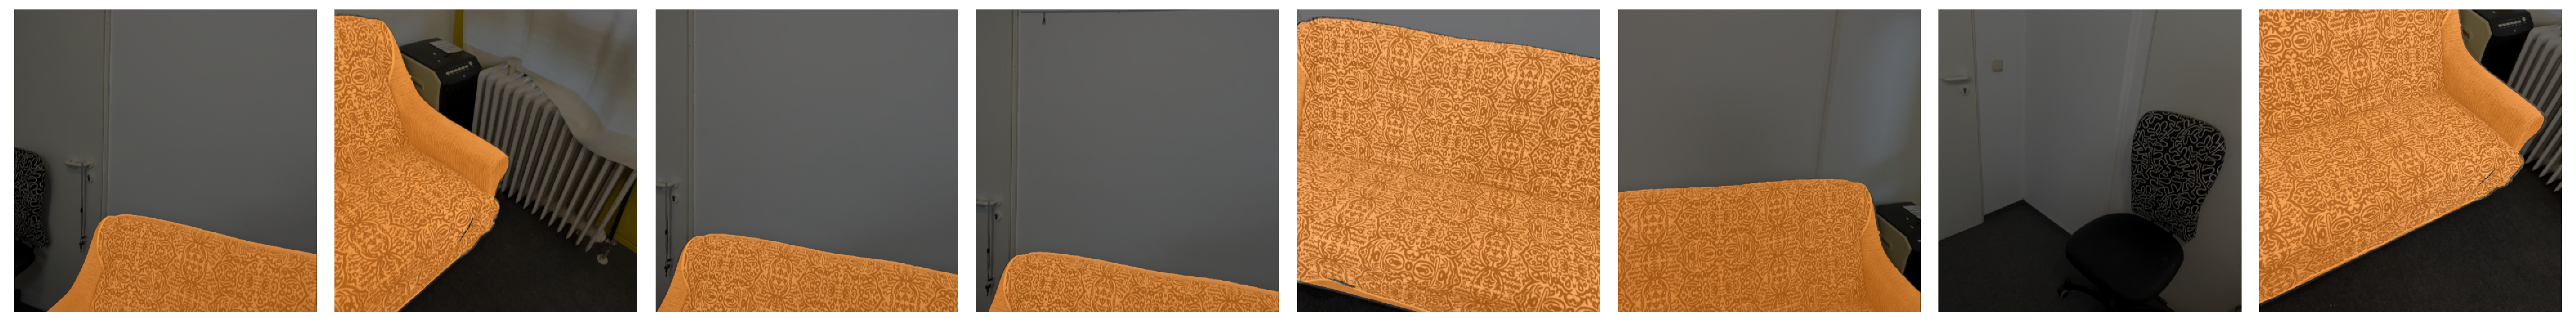
\includegraphics[width=\linewidth]{figs/scanpp_sample_no_fov_sampling.pdf}
    \captionsetup{justification=raggedright,singlelinecheck=false}
    \caption{\centering 不考虑视场的朴素随机采样}
    \label{fig:rand-samp}
  \end{minipage}
  \begin{minipage}{0.32\textwidth}
    \centering
    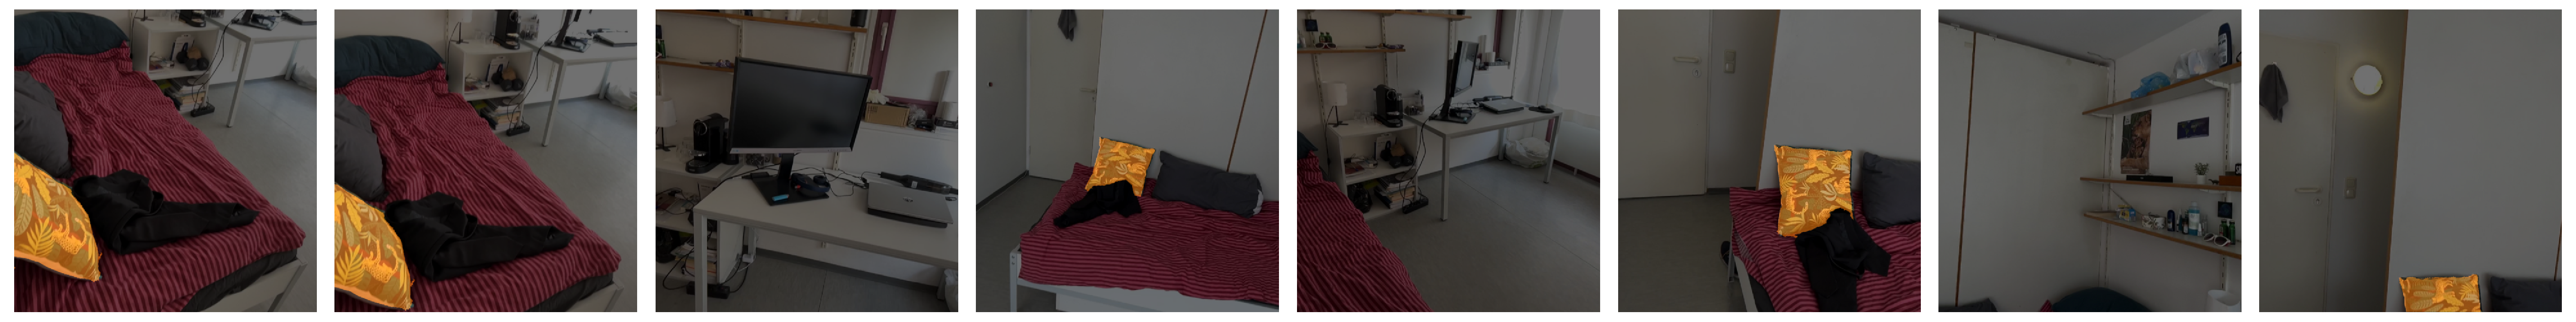
\includegraphics[width=\linewidth]{figs/scanpp_sample_fov_sampling.pdf}
    \captionsetup{justification=raggedright,singlelinecheck=false}
    \caption{\centering 视场感知采样策略（本文）}
    \label{fig:fov-samp}
  \end{minipage}
  \caption{\textbf{训练阶段采样策略概览。}
    (a) 连续采样只能覆盖相邻视角，跨视角变化有限。
    (b) 朴素随机采样会选择同一大型对象上空间上相距很远的区域。
    例如，帧~0 看到沙发左侧，而帧~1 看到右侧。
    由于这些区域在 3D 空间中距离很远，将它们作为相同监督信号会迫使模型匹配不一致的几何，从而导致学习歧义。
    (c) 我们的视场感知采样仅保留被掩码覆盖的 3D 点有足够比例落在参考相机视锥内的帧，在保留自然姿态和遮挡变化的同时，保证一致的几何重叠。}

  \label{fig:pipeline}
\vspace{-3mm}
\end{figure*}


训练模型的一个关键挑战是记忆模块容量有限（SAM2 最多保留八个记忆槽）。
为了让模型学习跨多样相机视角的鲁棒对象识别，我们必须谨慎设计如何从每个视频序列采样训练帧。

\vspace{-1em}
\subsubsection{朴素随机采样。}
一种直接策略是如 \cref{fig:rand-samp} 所示，从视频中随机采样 $N$ 帧。
这会让模型接触到广泛的相机视角和对象外观分布。
随机采样也会自然引入场景中的干扰物或视觉相似对象，从而鼓励模型依赖 3D 感知对齐，而非纯局部 2D 相似性。

\vspace{-1em}
\subsubsection{对象跨越问题。}
然而，当对象占据较大空间范围时，朴素随机采样会引入一种失败模式。
以床、桌子或柜子为例：两个随机采样帧可能都包含同一实例，却对应空间上相距很远的区域（例如一帧位于床头，另一帧位于床尾）。
我们的目标是施加 3D 位置一致性，即鼓励模型通过识别对象处在邻近 3D 位置来定位对象；因此，大型对象的这些宽基线视图可能与预期训练信号相矛盾。
尽管两个帧属于同一实例，它们投影出的 3D 位置却相距很远，这会混淆学习目标。

\vspace{-1em}
\subsubsection{视场采样。}
在每次训练迭代中，第一个采样帧被指定为参考帧。
为选择剩余 $N\!-\!1$ 帧，我们使用相机位姿和深度施加基于 FOV 的过滤。
对于每个候选帧，我们将其对象掩码反投影到 3D，将点变换到参考帧坐标系，并重新投影到参考图像。
只有当其被掩码覆盖的 3D 点有足够比例落在参考相机视锥内时，该帧才会被保留：
\[
\frac{\#\{\text{候选帧掩码点位于参考视锥内}\}}
       {\#\{\text{候选帧中的掩码点}\}}
> \tau.
\]
这确保所选帧观察到对象的重叠物理区域，避免同一实例的两个视角对应远距离、非重叠部分的退化情形。
我们不会过滤掉部分遮挡帧：视锥重叠反映的是观察方向上的对齐，而非完全可见；保留遮挡情况有助于模型学习区分视角变化和真实对象缺失。

需要注意的是，我们仅在候选掩码包含对象时将 FoV Sampling 作为过滤器。对于训练中也会采样到的无对象帧，模型只需预测目标不存在。在这些情况下，空间距离不会影响目标函数。也就是说，当视角相距很远时，预测由几何不一致驱动；而对于相邻视角，预测则依赖外观线索。

我们的最终采样策略及其消融实验见 \cref{sec:exp}。

\vspace{-0.5em}
\subsection{动态对象回退}
\vspace{-0.5em}
我们方法的一个直观限制在于动态对象，其形状、位置或方向可能随时间变化。这类场景在传统 VOS 基准中很常见~\cite{perazzi2017davis, xu2018youtube, fan2019lasot}。
我们的方法很大程度上依赖对象相对于周围几何的相对外观（即跨视角一致的几何位置）。
当对象发生显著运动时，这一假设可能被破坏，从而导致跟踪失败。
为解决该问题，我们使用~\cite{Huang_2025_seganymotion} 检测运动存在；一旦观察到显著运动，就回退到原始 SAM2 流水线。
由于在我们的框架中 SAM2 图像编码器保持冻结，我们可以复用视觉特征，记忆注意力和掩码解码器带来的额外计算开销可以忽略。

经验上，我们观察到在序列中途动态切换 3AM 和原始 SAM2（例如在掩码解码器之前加入简单运动检测分支）会破坏时间记忆库，因为两条路径产生的掩码分布本质不同。因此，当检测到显著运动时，我们采用简单的序列级回退到原始 SAM2 流水线。
这一设计基于对跟踪场景的实用分类，即根据对象相对于相机视锥的可见性划分：
(1) \textit{持续可见的动态对象}，对象始终位于相机视锥内，原始 SAM2 表现良好；
(2) \textit{短暂消失的静态对象}，对象离开相机视锥后再次进入，形成 3AM 旨在解决的重识别问题；以及
(3) \textit{视锥外发生未观测运动的动态对象}。

第三种情形本质上是病态问题，因为对象在相机视锥外未被观测时可能不可预测地移动。因此，可靠跟踪在根本上是不可能的。既然这种极端场景无法有效解决，就没有必要设计复杂的序列中途融合模块。
因此，一个简单的序列级切换足以覆盖两个可处理场景。
